\section{Supplementary Notes}

\subsection{Overview of Supplementary Data}
This section provides additional derivations and empirical results supporting the main text. Citations within the supplement are managed by a separate \texttt{refsection}, ensuring that references like \cite{novembre2008genes} appear in the supplementary bibliography.

\subsection{Derivation of the Test Statistic}
We define the standardized $Z$-score for the estimated effect size $\hat{\beta}$ as:
\begin{equation}
    Z = \frac{\hat{\beta}}{\text{SE}(\hat{\beta})}
    \label{eq:zscore}
\end{equation}
Note that \cref{eq:zscore} follows the "S" numbering convention (e.g., Equation S1) defined in our template.

\subsection{Supplementary Tables and Figures}

% Example of a Supplementary Table
\begin{table}[h]
    \centering
    \caption{Summary of notation used in the supplementary analysis.}
    \begin{tabular}{@{}ll@{}}
        \toprule
        Symbol & Description \\
        \midrule
        $\bbeta$ & Vector of effect sizes \\
        $\bSigma$ & Covariance matrix \\
        $n$ & Sample size \\
        \bottomrule
    \end{tabular}
    \label{tab:supp_notation}
\end{table}

As shown in \cref{tab:supp_notation}, we maintain consistency with the notation used in the primary Methods section.

\rmk{Note: If you have large figures with multiple panels, use the subcaption package features defined in your preamble.}

\begin{figure}[h]
    \centering
    % \includegraphics[width=0.8\textwidth]{suppl_figs/sim_result_v1} 
    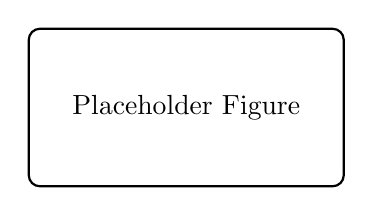
\begin{tikzpicture}
        \draw[thick, rounded corners] (0,0) rectangle (4,2) node[midway]{Placeholder Figure};
    \end{tikzpicture}
    \caption{Validation of the model under null conditions. This figure will be labeled as \textbf{Figure S1}.}
    \label{fig:supp_sim}
\end{figure}

\cref{fig:supp_sim} demonstrates the robustness of our $Z$-score calculation across different variance scales.